\documentclass[a4paper,12pt]{article}
\DeclareMathSizes{12}{30}{16}{12}

\usepackage[T1]{fontenc}
\usepackage[utf8]{inputenc}
\usepackage[english]{babel}

\usepackage[margin=3cm]{geometry}
\usepackage{graphicx}
\usepackage{float}
\usepackage{blindtext}
\usepackage{titling}
\usepackage{titlesec}
\usepackage[center]{caption}
\usepackage{wrapfig}
\usepackage{animate}
\usepackage{enumitem}
\setlist[enumerate]{itemsep=0mm}


\titleformat{\section}
{\Large\bfseries}
% {\Roman{section}.}
{\thesection.}
{0.5em}
{}

\titleformat{\subsection}
{\center\large\bfseries}
% {\Roman{subsection}}
{\thesubsection}
{0.5em}
{}

\titlespacing{\subsection}
{2em}{2.5em}{0.5em}

\title{Využití umělé inteligence a genetického algoritmu pro autonomní řízení}
\author{Marek Bečvář}
\date{Červen 2020}

\renewcommand{\maketitle}
{
    \begin{center}
        \vspace*{0cm}
        \LARGE{\textbf{\thetitle}}\\
        \vspace{0.5cm}
        \Large{\textbf{\theauthor}}\\
        \vspace{0.5cm}
        \normalsize{\thedate}
        \vspace{0.2cm}
        \hrule
    \end{center}
}

\addto\captionsenglish{\renewcommand{\figurename}{Schéma}}

\newcommand{\tab}
{
    \hspace*{1em}
}

\linespread{1.25}
\begin{document}
    \maketitle

    \vspace{0.25cm}
    \section{O projektu}
        \tab Tento projekt byl zpracován v roce 2020 jako maturitní práce 6.ročníku 
        víceletého gymnázia Boženy Němcové v Hradci Králové.\\
        \tab Hlavní myšlenkou je využití strojového učení umělé inteligence genetickým 
        algoritmem s cílem projetí uživatelem nastavené tratě. Výsledek snažení 
        je postupně promítán do grafu. Schopnost by se měla, i po dosažení cíle (projetí tratí),
        stále rozvíjet.

    \section{Mechanismy programu}
    \subsection{Umělá inteligence}
        Pojem \textbf{umělé inteligence} je dnes člověku prezentován v trochu zkreslené formě.
        Lidem se mohou vybavit některé sci-fi filmové scény s roboty, ale to není úplně přesné.
        Ve slově \textit{inteligence} se doopravdy skrývá řada výpočtů zpracovávajících vstupní data 
        na požadovaný výstup. Tyto výpočty se provádějí v předem definované 
        struktuře tzv. \textbf{neuronové sítě}.\\
            
        \begin{figure}[H]
        \centering
        \begin{minipage}[t]{.5\textwidth}
            \centering
            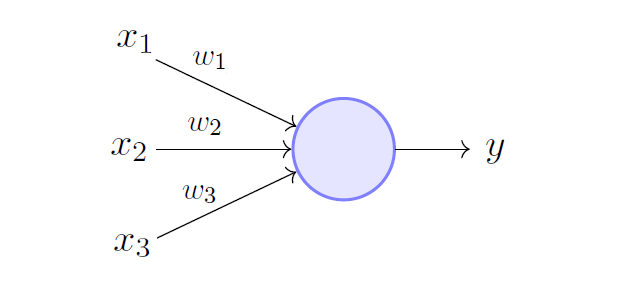
\includegraphics[width=0.9\linewidth]{data/perceptron-model1.png}
            \captionof{figure}{Perceptron}
            \label{fig:perceptron}
        \end{minipage}%
        \begin{minipage}[t]{.5\textwidth}
            \centering
            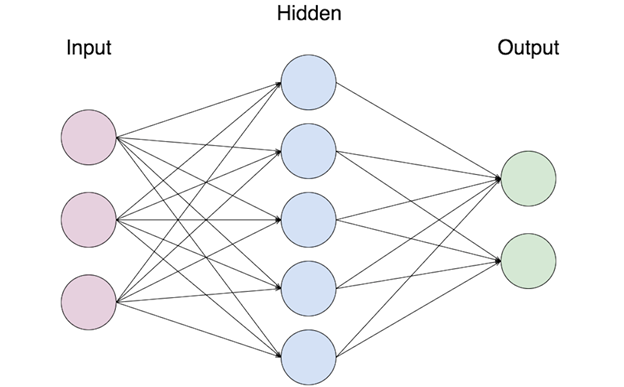
\includegraphics[width=0.85\linewidth]{data/easynn-scheme.png}
            \captionof{figure}{Neuronová síť}
            \label{fig:easynn}
        \end{minipage}
        \end{figure}

        Neuronová síť je modelována s inspirací v mozkových neuronech. Každý bod je považován za
        samostatný neuron a má řadu spojení, z biologie \textit{axonů}. Právě tato spojení jsou důležitou
        funkční složkou neuronových sítí. V programu tedy vždy uchováváme číselnou hodnotu každého z nich.
        Tato hodnota je obvykle reálné číslo v rozsahu od -1.0 do 1.0.
        Neurony dělíme do vrstev (VSTUP, SKRYTÁ, VÝSTUP). Data ze sledovaného prostředí přenášíme
        do vstupní vrstvy a výsledek pozoruje na vrstvě výstupní. Existuje pravidlo, že každý neuron z nižší vrstvy 
        je spojen se všemi neurony ve vyšší vrstvě. Nejjednodušším znázorněním neuronu je 
        Schéma~\ref{fig:perceptron}, skládající se z 3 vstupů a 1 výstupu.
        Jak se ale tvoří číselné hodnoty?

        \begin{equation}
            \sigma(\displaystyle\sum_{k=1}^{n}{x_k * w_k})
        \end{equation}
        \begin{equation}
            \scriptscriptstyle 0.5*0.1 + 1.0*0.5 + 0.25*0.3 = 0.625 \hspace*{0.2cm} \rightarrow \hspace*{0.2cm}
            \sigma(0.625)=0.625
        \end{equation}

        kde $\scriptstyle \sigma$ je \textit{aktivační funkce}. Tyto funkce pouze upravují 
        možný rozsah výstupních hodnot. Takto získáme finální hodnotu na jednom neuronu.\\

        \begin{wrapfigure}[5]{r}{0.4\textwidth}
            \vspace{-2.5em}
            \centering
            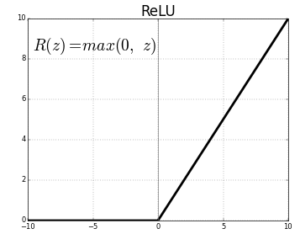
\includegraphics[width=0.8\linewidth]{data/relu.png}
            \caption{RELU aktivační funkce} 
            \label{fig:relu}
        \end{wrapfigure}

        Příkladem takové aktivační funkce může být třeba \textbf{RELU} (Rectified Linear Unit).
        Ta výstupní hodnoty změní tak, že kladné nechá beze změny a záporné změní na nulu.
        Tyto změny pomáhají při přenosu signálu mezi neurony v síti.
        \\\\\\\\
        \begin{flushleft}
            \vspace{-3em}
            Složitější neuronové sítě jsou už jen opakováním tohoto zavedeného postupu. Dále se pro sítě 
            tohoto typu zavádí jméno \textbf{hluboká neuronová síť} (\textit{z ang. deep neural network}). 
            To označuje schéma, ve kterém je použita více než jedna skrytá vrstva.
        \end{flushleft}

        \begin{figure}[H]
            \centering
            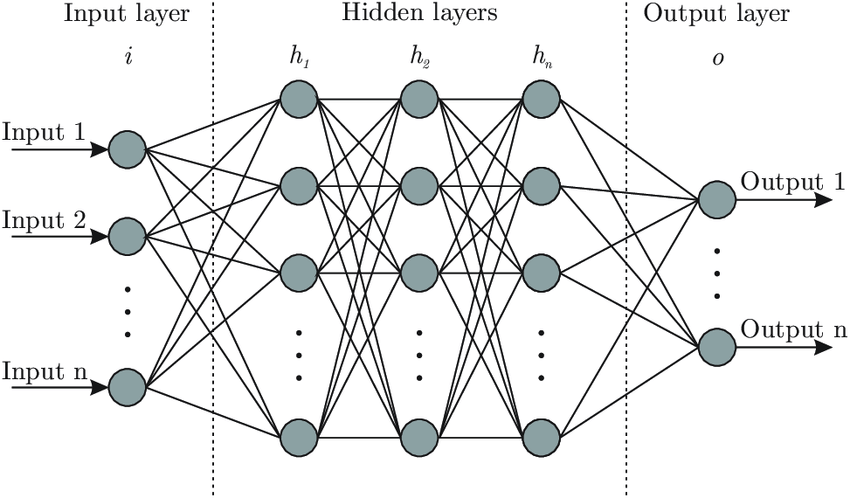
\includegraphics[width=0.54\textwidth]{data/nn-scheme.png}
            \captionof{figure}{Hluboká neuronová síť}
            \label{fig:deepnn}
        \end{figure}

        Při práci s neuronovými sítěmi, abychom zvětšili přesnost výpočtů, upravujeme vstupy
        (první řadu neuronů) do určitého číselného rozsahu. Poté necháme proběhnout všechny 
        matematické operace uvnitř sítě a sledujeme výsledek. To jak se program bude při daném 
        výsledku chovat je opět pouze na volbě autora programu.\\\\
        \tab Poté nastává \textbf{proces učení}, při kterém upravujeme hodnoty všech spojení v síti tak,
        aby při určitých vstupních hodnotách nastal požadovaný výstup. Pro učení existuje řada algoritmů
        založených na různých matematických úpravách. Pro moji síť jsem ale zvolil postup učení,
        inspirovaný přírodou, tzv. \textbf{genetický algoritmus} (\textit{"O původu druhů" Charles Darwin - evoluční teorie}).\\\\
        \tab Samotná architektura (počet neuronů v každé z vrstev) je pro funkčnost velmi
        důležitá a neexistuje předem daný, jednoznačně správný postup. Tato část je tedy často o 
        spoustě drobných úprav při hledání dobře pracující sítě.\\
        \tab Architektura, která je použita v prezentovaném programu, byla docílena řadou testů
        různých sítí proti sobě.\\\\
        \tab\textbf{Finální síť použitá v programu je ve schématu [6, 8, 4, 2]}\\
        5 vstupů měřících vzdálenost + 1 vstup měřící čas\\
        1 výstup pro rychlost + 1 výstup pro zatáčení

    \subsection{Genetický algoritmus}
        Genetický algoritmus má v informatice mnoho využití při řešení logických problémů. 
        Ve svém projektu jsem ho použil na úpravu spojů v neuronové síti. Algoritmus je také známý svými 
        procesy, které přímo kopírují fungování v přírodě. Teorie genetického algoritmu je založena 
        na Darwinově teorii \textit{"O původu druhů"}\\
        \tab Rozlišujeme jedince, jejichž genetickou informací jsou všechny hodnoty spojů v neuronové síti. 
        Při učení procházíme stálým cyklem, při kterém se tato genetická informace upravuje tak, 
        aby se výsledky zlepšovaly.
        \vspace{0.5cm}
        \begin{figure}[H]
            \centering
            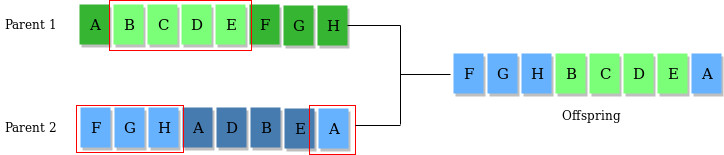
\includegraphics[width=0.8\textwidth]{data/genetic-algorithm.png}
            \captionof{figure}{Genetický crossover}
            \label{fig:crossover}
        \end{figure}

        \underline{\textbf{\large{Cyklus genetického algoritmu}}}
        \begin{enumerate}[itemsep=-1.5mm]
            \item Určíme, jak velký počet jedinců chceme testovat (\textbf{velikost populace})
            \item Naplníme populaci náhodně generovanými jedinci
            \begin{itemize}[noitemsep]
                \item každý jedinec je abstrakcí jedné náhodné neuronové sítě
                \item všechna spojení sítě tvoří genetickou informaci
            \end{itemize}
            \item Celou populaci vyzkoušíme v testovacím prostředí a zapíšeme jejich \textbf{zdatnost} 
                v zadaném problému
            \item Z populace pseudo-náhodně vybereme skupinu rodičů nové generace 
            \begin{itemize}[noitemsep]
                \item ti s \textbf{vyšší zdatností mají větší šanči} být zvoleni mezi rodiče
                \item každý z jedinců může být zvolen opakovaně
            \end{itemize}
            \item Ze skupiny rodičů náhodně vybereme vždy dva jedince a náhodným poskládáním jejich
                genetických informací vytvoříme dva nové potomky (\textbf{genetický crossover} Schéma~\ref{fig:crossover})
            \item Každý gen každého potomka má určitou šanci náhodně zmutovat
            \begin{itemize}[noitemsep]
                \item hodnotu této náhody musíme určit
                \item \textbf{pravděpodobnost mutace} se obvykle pohybuje mezi 1\% - 5\%\\
                    Příliš malá hodnota a populace není schopna prozkoumávat nová řešení.
                    Příliš velká hodnota a mutace může rozbít správná řešení.

            \end{itemize}
            \item Do splnění požadavků opakujeme kroky 3 - 6, při kterých by se měli 
                objevovat stále lepší a lepší jedinci.
        \end{enumerate}
        \hrule

        \vspace{0.75cm}
        Základní myšlenkou při křížení genetických informací je předpoklad, že ze dvou úspěšných
        jedinců vznike vždy potomek buď \textbf{zdatnější, nebo stejně dobrý}.\\
        V praxi toto není vždy pravda, už kvůli přítomnosti náhody ve většině krocích cyklu. 
        Teorie ale funguje, a tak jsme tímto způsobem schopni dojít správných výsledků.
        \\

        V projektu je genetický algoritmus založen s populací o \textbf{50 členech}. 
        Každý člen představuje náhodnou neuronovou síť (stejné architektury [6, 8, 4, 2]).
        Kvůli zdánlivé obtížnosti úkolu a velikosti sítě jsem se rozhodl pro hodnotu 
        \textbf{pravděpodobnosti mutace = 2,5\%}. Zároveň pro snazší uchování nejlepší 
        genetické informace se nejlepší jedinec poslední generace přenáší do další.
        
\end{document}
